\documentclass[1p]{elsarticle_modified}
%\bibliographystyle{elsarticle-num}

%\usepackage[colorlinks]{hyperref}
%\usepackage{abbrmath_seonhwa} %\Abb, \Ascr, \Acal ,\Abf, \Afrak
\usepackage{amsfonts}
\usepackage{amssymb}
\usepackage{amsmath}
\usepackage{amsthm}
\usepackage{scalefnt}
\usepackage{amsbsy}
\usepackage{kotex}
\usepackage{caption}
\usepackage{subfig}
\usepackage{color}
\usepackage{graphicx}
\usepackage{xcolor} %% white, black, red, green, blue, cyan, magenta, yellow
\usepackage{float}
\usepackage{setspace}
\usepackage{hyperref}

\usepackage{tikz}
\usetikzlibrary{arrows}

\usepackage{multirow}
\usepackage{array} % fixed length table
\usepackage{hhline}

%%%%%%%%%%%%%%%%%%%%%
\makeatletter
\renewcommand*\env@matrix[1][\arraystretch]{%
	\edef\arraystretch{#1}%
	\hskip -\arraycolsep
	\let\@ifnextchar\new@ifnextchar
	\array{*\c@MaxMatrixCols c}}
\makeatother %https://tex.stackexchange.com/questions/14071/how-can-i-increase-the-line-spacing-in-a-matrix
%%%%%%%%%%%%%%%

\usepackage[normalem]{ulem}

\newcommand{\msout}[1]{\ifmmode\text{\sout{\ensuremath{#1}}}\else\sout{#1}\fi}
%SOURCE: \msout is \stkout macro in https://tex.stackexchange.com/questions/20609/strikeout-in-math-mode

\newcommand{\cancel}[1]{
	\ifmmode
	{\color{red}\msout{#1}}
	\else
	{\color{red}\sout{#1}}
	\fi
}

\newcommand{\add}[1]{
	{\color{blue}\uwave{#1}}
}

\newcommand{\replace}[2]{
	\ifmmode
	{\color{red}\msout{#1}}{\color{blue}\uwave{#2}}
	\else
	{\color{red}\sout{#1}}{\color{blue}\uwave{#2}}
	\fi
}

\newcommand{\Sol}{\mathcal{S}} %segment
\newcommand{\D}{D} %diagram
\newcommand{\A}{\mathcal{A}} %arc


%%%%%%%%%%%%%%%%%%%%%%%%%%%%%5 test

\def\sl{\operatorname{\textup{SL}}(2,\Cbb)}
\def\psl{\operatorname{\textup{PSL}}(2,\Cbb)}
\def\quan{\mkern 1mu \triangleright \mkern 1mu}

\theoremstyle{definition}
\newtheorem{thm}{Theorem}[section]
\newtheorem{prop}[thm]{Proposition}
\newtheorem{lem}[thm]{Lemma}
\newtheorem{ques}[thm]{Question}
\newtheorem{cor}[thm]{Corollary}
\newtheorem{defn}[thm]{Definition}
\newtheorem{exam}[thm]{Example}
\newtheorem{rmk}[thm]{Remark}
\newtheorem{alg}[thm]{Algorithm}

\newcommand{\I}{\sqrt{-1}}
\begin{document}

%\begin{frontmatter}
%
%\title{Boundary parabolic representations of knots up to 8 crossings}
%
%%% Group authors per affiliation:
%\author{Yunhi Cho} 
%\address{Department of Mathematics, University of Seoul, Seoul, Korea}
%\ead{yhcho@uos.ac.kr}
%
%
%\author{Seonhwa Kim} %\fnref{s_kim}}
%\address{Center for Geometry and Physics, Institute for Basic Science, Pohang, 37673, Korea}
%\ead{ryeona17@ibs.re.kr}
%
%\author{Hyuk Kim}
%\address{Department of Mathematical Sciences, Seoul National University, Seoul 08826, Korea}
%\ead{hyukkim@snu.ac.kr}
%
%\author{Seokbeom Yoon}
%\address{Department of Mathematical Sciences, Seoul National University, Seoul, 08826,  Korea}
%\ead{sbyoon15@snu.ac.kr}
%
%\begin{abstract}
%We find all boundary parabolic representation of knots up to 8 crossings.
%
%\end{abstract}
%\begin{keyword}
%    \MSC[2010] 57M25 
%\end{keyword}
%
%\end{frontmatter}

%\linenumbers
%\tableofcontents
%
\newcommand\colored[1]{\textcolor{white}{\rule[-0.35ex]{0.8em}{1.4ex}}\kern-0.8em\color{red} #1}%
%\newcommand\colored[1]{\textcolor{white}{ #1}\kern-2.17ex	\textcolor{white}{ #1}\kern-1.81ex	\textcolor{white}{ #1}\kern-2.15ex\color{red}#1	}

{\Large $\underline{11a_{153}~(K11a_{153})}$}

\setlength{\tabcolsep}{10pt}
\renewcommand{\arraystretch}{1.6}
\vspace{1cm}\begin{tabular}{m{100pt}>{\centering\arraybackslash}m{274pt}}
\multirow{5}{120pt}{
	\centering
	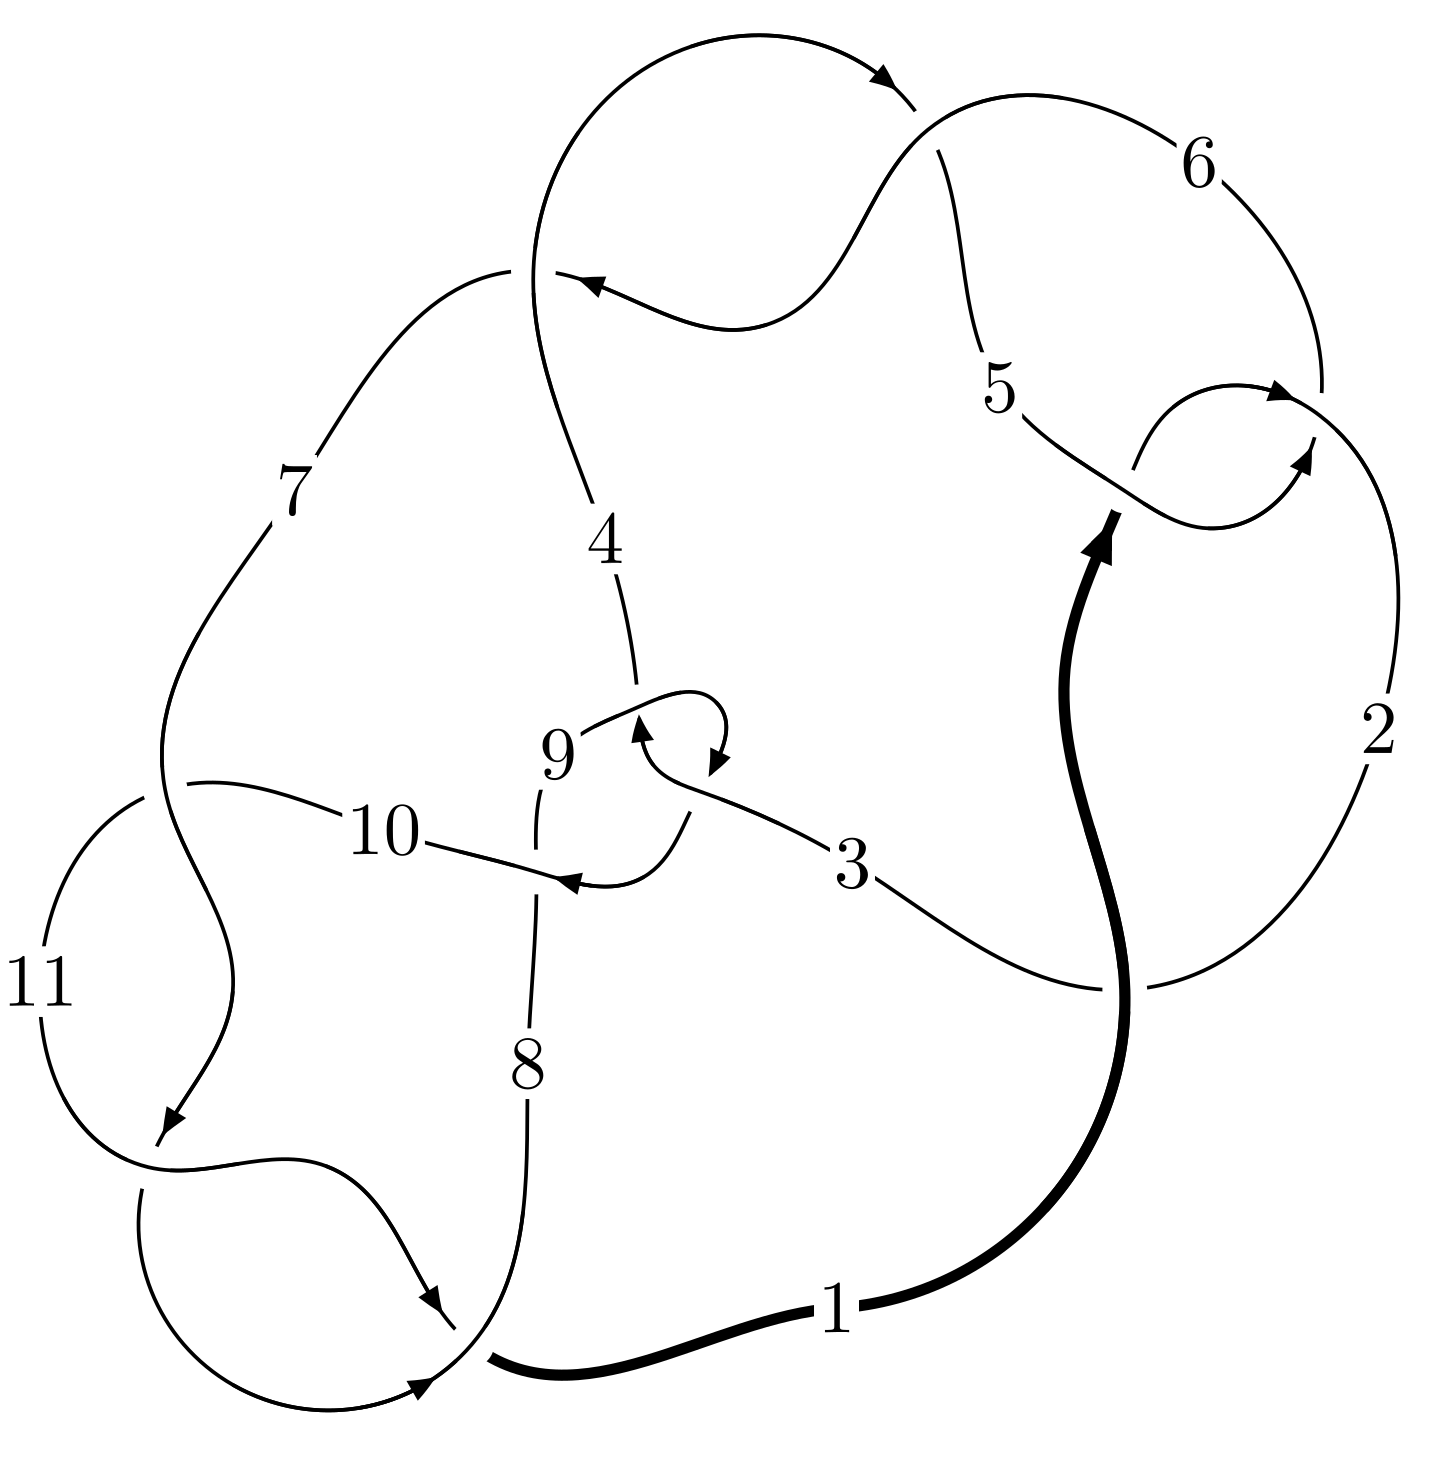
\includegraphics[width=112pt]{../../../GIT/diagram.site/Diagrams/png/402_11a_153.png}\\
\ \ \ A knot diagram\footnotemark}&
\allowdisplaybreaks
\textbf{Linearized knot diagam} \\
\cline{2-2}
 &
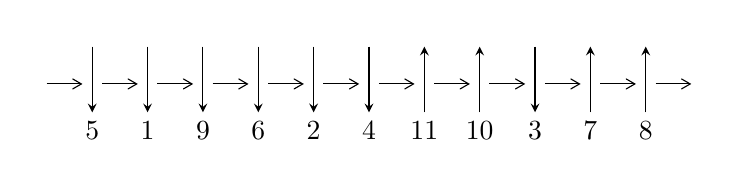
\begin{tikzpicture}[x=20pt, y=17pt]
	% nodes
	\node (C0) at (0, 0) {};
	\node (C1) at (1, 0) {};
	\node (C1U) at (1, +1) {};
	\node (C1D) at (1, -1) {5};

	\node (C2) at (2, 0) {};
	\node (C2U) at (2, +1) {};
	\node (C2D) at (2, -1) {1};

	\node (C3) at (3, 0) {};
	\node (C3U) at (3, +1) {};
	\node (C3D) at (3, -1) {9};

	\node (C4) at (4, 0) {};
	\node (C4U) at (4, +1) {};
	\node (C4D) at (4, -1) {6};

	\node (C5) at (5, 0) {};
	\node (C5U) at (5, +1) {};
	\node (C5D) at (5, -1) {2};

	\node (C6) at (6, 0) {};
	\node (C6U) at (6, +1) {};
	\node (C6D) at (6, -1) {4};

	\node (C7) at (7, 0) {};
	\node (C7U) at (7, +1) {};
	\node (C7D) at (7, -1) {11};

	\node (C8) at (8, 0) {};
	\node (C8U) at (8, +1) {};
	\node (C8D) at (8, -1) {10};

	\node (C9) at (9, 0) {};
	\node (C9U) at (9, +1) {};
	\node (C9D) at (9, -1) {3};

	\node (C10) at (10, 0) {};
	\node (C10U) at (10, +1) {};
	\node (C10D) at (10, -1) {7};

	\node (C11) at (11, 0) {};
	\node (C11U) at (11, +1) {};
	\node (C11D) at (11, -1) {8};
	\node (C12) at (12, 0) {};

	% arrows
	\draw[->,>={angle 60}]
	(C0) edge (C1) (C1) edge (C2) (C2) edge (C3) (C3) edge (C4) (C4) edge (C5) (C5) edge (C6) (C6) edge (C7) (C7) edge (C8) (C8) edge (C9) (C9) edge (C10) (C10) edge (C11) (C11) edge (C12) ;	\draw[->,>=stealth]
	(C1U) edge (C1D) (C2U) edge (C2D) (C3U) edge (C3D) (C4U) edge (C4D) (C5U) edge (C5D) (C6U) edge (C6D) (C7D) edge (C7U) (C8D) edge (C8U) (C9U) edge (C9D) (C10D) edge (C10U) (C11D) edge (C11U) ;
	\end{tikzpicture} \\
\hhline{~~} \\& 
\textbf{Solving Sequence} \\ \cline{2-2} 
 &
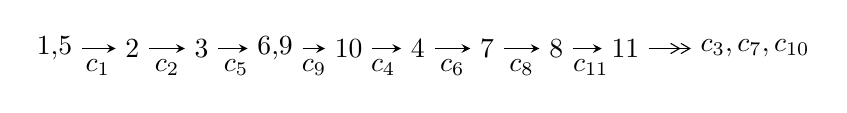
\begin{tikzpicture}[x=25pt, y=7pt]
	% node
	\node (A0) at (-1/8, 0) {1,5};
	\node (A1) at (1, 0) {2};
	\node (A2) at (2, 0) {3};
	\node (A3) at (49/16, 0) {6,9};
	\node (A4) at (33/8, 0) {10};
	\node (A5) at (41/8, 0) {4};
	\node (A6) at (49/8, 0) {7};
	\node (A7) at (57/8, 0) {8};
	\node (A8) at (65/8, 0) {11};
	\node (C1) at (1/2, -1) {$c_{1}$};
	\node (C2) at (3/2, -1) {$c_{2}$};
	\node (C3) at (5/2, -1) {$c_{5}$};
	\node (C4) at (29/8, -1) {$c_{9}$};
	\node (C5) at (37/8, -1) {$c_{4}$};
	\node (C6) at (45/8, -1) {$c_{6}$};
	\node (C7) at (53/8, -1) {$c_{8}$};
	\node (C8) at (61/8, -1) {$c_{11}$};
	\node (A9) at (10, 0) {$c_{3},c_{7},c_{10}$};

	% edge
	\draw[->,>=stealth]	
	(A0) edge (A1) (A1) edge (A2) (A2) edge (A3) (A3) edge (A4) (A4) edge (A5) (A5) edge (A6) (A6) edge (A7) (A7) edge (A8) ;
	\draw[->>,>={angle 60}]	
	(A8) edge (A9);
\end{tikzpicture} \\ 

\end{tabular} \\

\footnotetext{
The image of knot diagram is generated by the software ``\textbf{Draw programme}" developed by Andrew Bartholomew(\url{http://www.layer8.co.uk/maths/draw/index.htm\#Running-draw}), where we modified some parts for our purpose(\url{https://github.com/CATsTAILs/LinksPainter}).
}\phantom \\ \newline 
\centering \textbf{Ideals for irreducible components\footnotemark of $X_{\text{par}}$} 
 
\begin{align*}
I^u_{1}&=\langle 
- u^{45}+u^{44}+\cdots+5 u^4+b,\;- u^{43}+6 u^{41}+\cdots-5 u^3+a,\;u^{47}-2 u^{46}+\cdots+2 u^2-1\rangle \\
I^u_{2}&=\langle 
b-1,\;a- u,\;u^3+u^2-1\rangle \\
\\
\end{align*}
\raggedright * 2 irreducible components of $\dim_{\mathbb{C}}=0$, with total 50 representations.\\
\footnotetext{All coefficients of polynomials are rational numbers. But the coefficients are sometimes approximated in decimal forms when there is not enough margin.}
\newpage
\renewcommand{\arraystretch}{1}
\centering \section*{I. $I^u_{1}= \langle - u^{45}+u^{44}+\cdots+5 u^4+b,\;- u^{43}+6 u^{41}+\cdots-5 u^3+a,\;u^{47}-2 u^{46}+\cdots+2 u^2-1 \rangle$}
\flushleft \textbf{(i) Arc colorings}\\
\begin{tabular}{m{7pt} m{180pt} m{7pt} m{180pt} }
\flushright $a_{1}=$&$\begin{pmatrix}1\\0\end{pmatrix}$ \\
\flushright $a_{5}=$&$\begin{pmatrix}0\\u\end{pmatrix}$ \\
\flushright $a_{2}=$&$\begin{pmatrix}1\\u^2\end{pmatrix}$ \\
\flushright $a_{3}=$&$\begin{pmatrix}- u^2+1\\u^2\end{pmatrix}$ \\
\flushright $a_{6}=$&$\begin{pmatrix}- u\\- u^3+u\end{pmatrix}$ \\
\flushright $a_{9}=$&$\begin{pmatrix}u^{43}-6 u^{41}+\cdots-4 u^5+5 u^3\\u^{45}- u^{44}+\cdots+5 u^5-5 u^4\end{pmatrix}$ \\
\flushright $a_{10}=$&$\begin{pmatrix}2 u^{46}-2 u^{45}+\cdots- u+1\\- u^{46}+u^{45}+\cdots+u^2+u\end{pmatrix}$ \\
\flushright $a_{4}=$&$\begin{pmatrix}u^3\\u^5- u^3+u\end{pmatrix}$ \\
\flushright $a_{7}=$&$\begin{pmatrix}- u^5- u\\- u^7+u^5-2 u^3+u\end{pmatrix}$ \\
\flushright $a_{8}=$&$\begin{pmatrix}- u^{44}+u^{43}+\cdots+5 u^3- u^2\\- u^{46}+u^{45}+\cdots-9 u^4+u^2\end{pmatrix}$ \\
\flushright $a_{11}=$&$\begin{pmatrix}u^{46}- u^{45}+\cdots- u+1\\- u^{46}+u^{45}+\cdots+u^2+u\end{pmatrix}$\\ \flushright $a_{11}=$&$\begin{pmatrix}u^{46}- u^{45}+\cdots- u+1\\- u^{46}+u^{45}+\cdots+u^2+u\end{pmatrix}$\\&\end{tabular}
\flushleft \textbf{(ii) Obstruction class $= -1$}\\~\\
\flushleft \textbf{(iii) Cusp Shapes $= - u^{46}+2 u^{45}+\cdots-11 u-3$}\\~\\
\newpage\renewcommand{\arraystretch}{1}
\flushleft \textbf{(iv) u-Polynomials at the component}\newline \\
\begin{tabular}{m{50pt}|m{274pt}}
Crossings & \hspace{64pt}u-Polynomials at each crossing \\
\hline $$\begin{aligned}c_{1},c_{5}\end{aligned}$$&$\begin{aligned}
&u^{47}+2 u^{46}+\cdots-2 u^2+1
\end{aligned}$\\
\hline $$\begin{aligned}c_{2},c_{4},c_{6}\end{aligned}$$&$\begin{aligned}
&u^{47}+12 u^{46}+\cdots+4 u+1
\end{aligned}$\\
\hline $$\begin{aligned}c_{3},c_{9}\end{aligned}$$&$\begin{aligned}
&u^{47}+u^{46}+\cdots+28 u+8
\end{aligned}$\\
\hline $$\begin{aligned}c_{7},c_{10},c_{11}\end{aligned}$$&$\begin{aligned}
&u^{47}+4 u^{46}+\cdots+5 u+1
\end{aligned}$\\
\hline $$\begin{aligned}c_{8}\end{aligned}$$&$\begin{aligned}
&u^{47}-21 u^{46}+\cdots-112 u+64
\end{aligned}$\\
\hline
\end{tabular}\\~\\
\newpage\renewcommand{\arraystretch}{1}
\flushleft \textbf{(v) Riley Polynomials at the component}\newline \\
\begin{tabular}{m{50pt}|m{274pt}}
Crossings & \hspace{64pt}Riley Polynomials at each crossing \\
\hline $$\begin{aligned}c_{1},c_{5}\end{aligned}$$&$\begin{aligned}
&y^{47}-12 y^{46}+\cdots+4 y-1
\end{aligned}$\\
\hline $$\begin{aligned}c_{2},c_{4},c_{6}\end{aligned}$$&$\begin{aligned}
&y^{47}+48 y^{46}+\cdots-20 y-1
\end{aligned}$\\
\hline $$\begin{aligned}c_{3},c_{9}\end{aligned}$$&$\begin{aligned}
&y^{47}+21 y^{46}+\cdots-112 y-64
\end{aligned}$\\
\hline $$\begin{aligned}c_{7},c_{10},c_{11}\end{aligned}$$&$\begin{aligned}
&y^{47}-42 y^{46}+\cdots+53 y-1
\end{aligned}$\\
\hline $$\begin{aligned}c_{8}\end{aligned}$$&$\begin{aligned}
&y^{47}+5 y^{46}+\cdots+249088 y-4096
\end{aligned}$\\
\hline
\end{tabular}\\~\\
\newpage\flushleft \textbf{(vi) Complex Volumes and Cusp Shapes}
$$\begin{array}{c|c|c}  
\text{Solutions to }I^u_{1}& \I (\text{vol} + \sqrt{-1}CS) & \text{Cusp shape}\\
 \hline 
\begin{aligned}
u &= -0.951038 + 0.332468 I \\
a &= -0.548939 - 0.454811 I \\
b &= -1.39671 - 0.26399 I\end{aligned}
 & -2.29859 + 5.08605 I & -6.19055 - 7.78708 I \\ \hline\begin{aligned}
u &= -0.951038 - 0.332468 I \\
a &= -0.548939 + 0.454811 I \\
b &= -1.39671 + 0.26399 I\end{aligned}
 & -2.29859 - 5.08605 I & -6.19055 + 7.78708 I \\ \hline\begin{aligned}
u &= \phantom{-}1.011380 + 0.139586 I \\
a &= \phantom{-}0.187121 - 1.081320 I \\
b &= \phantom{-}0.152878 + 0.035343 I\end{aligned}
 & \phantom{-}1.25225 + 2.83779 I & -2.68977 - 2.39473 I \\ \hline\begin{aligned}
u &= \phantom{-}1.011380 - 0.139586 I \\
a &= \phantom{-}0.187121 + 1.081320 I \\
b &= \phantom{-}0.152878 - 0.035343 I\end{aligned}
 & \phantom{-}1.25225 - 2.83779 I & -2.68977 + 2.39473 I \\ \hline\begin{aligned}
u &= \phantom{-}0.896160 + 0.336643 I \\
a &= \phantom{-}0.608816 - 1.251080 I \\
b &= \phantom{-}0.208048 + 0.420593 I\end{aligned}
 & \phantom{-}0.73808 - 3.39872 I & -3.20420 + 5.17325 I \\ \hline\begin{aligned}
u &= \phantom{-}0.896160 - 0.336643 I \\
a &= \phantom{-}0.608816 + 1.251080 I \\
b &= \phantom{-}0.208048 - 0.420593 I\end{aligned}
 & \phantom{-}0.73808 + 3.39872 I & -3.20420 - 5.17325 I \\ \hline\begin{aligned}
u &= \phantom{-}0.929490 + 0.212978 I \\
a &= -0.382863 + 1.063800 I \\
b &= -0.152157 - 0.188016 I\end{aligned}
 & -2.99267 - 0.24824 I & -9.15885 + 0.73721 I \\ \hline\begin{aligned}
u &= \phantom{-}0.929490 - 0.212978 I \\
a &= -0.382863 - 1.063800 I \\
b &= -0.152157 + 0.188016 I\end{aligned}
 & -2.99267 + 0.24824 I & -9.15885 - 0.73721 I \\ \hline\begin{aligned}
u &= -1.006120 + 0.373819 I \\
a &= \phantom{-}0.507879 + 0.365560 I \\
b &= \phantom{-}1.365760 + 0.114872 I\end{aligned}
 & \phantom{-}2.62432 + 8.92326 I & -1.23068 - 8.39839 I \\ \hline\begin{aligned}
u &= -1.006120 - 0.373819 I \\
a &= \phantom{-}0.507879 - 0.365560 I \\
b &= \phantom{-}1.365760 - 0.114872 I\end{aligned}
 & \phantom{-}2.62432 - 8.92326 I & -1.23068 + 8.39839 I\\
 \hline 
 \end{array}$$\newpage$$\begin{array}{c|c|c}  
\text{Solutions to }I^u_{1}& \I (\text{vol} + \sqrt{-1}CS) & \text{Cusp shape}\\
 \hline 
\begin{aligned}
u &= -0.586342 + 0.704775 I \\
a &= \phantom{-}0.286240 - 0.496512 I \\
b &= -0.636220 - 0.653509 I\end{aligned}
 & \phantom{-}6.94014 + 2.76747 I & \phantom{-}5.54266 - 3.60808 I \\ \hline\begin{aligned}
u &= -0.586342 - 0.704775 I \\
a &= \phantom{-}0.286240 + 0.496512 I \\
b &= -0.636220 + 0.653509 I\end{aligned}
 & \phantom{-}6.94014 - 2.76747 I & \phantom{-}5.54266 + 3.60808 I \\ \hline\begin{aligned}
u &= -0.844254 + 0.267575 I \\
a &= \phantom{-}0.624042 + 0.701381 I \\
b &= \phantom{-}1.43152 + 0.59292 I\end{aligned}
 & \phantom{-}0.239586 + 1.107160 I & -2.87652 - 5.48870 I \\ \hline\begin{aligned}
u &= -0.844254 - 0.267575 I \\
a &= \phantom{-}0.624042 - 0.701381 I \\
b &= \phantom{-}1.43152 - 0.59292 I\end{aligned}
 & \phantom{-}0.239586 - 1.107160 I & -2.87652 + 5.48870 I \\ \hline\begin{aligned}
u &= -0.946938 + 0.664626 I \\
a &= -0.210609 - 0.192004 I \\
b &= -0.664543 + 0.135905 I\end{aligned}
 & \phantom{-}5.98354 + 2.31808 I & \phantom{-}4.28165 - 1.64217 I \\ \hline\begin{aligned}
u &= -0.946938 - 0.664626 I \\
a &= -0.210609 + 0.192004 I \\
b &= -0.664543 - 0.135905 I\end{aligned}
 & \phantom{-}5.98354 - 2.31808 I & \phantom{-}4.28165 + 1.64217 I \\ \hline\begin{aligned}
u &= -0.842514 + 0.793044 I \\
a &= -0.169363 + 0.125945 I \\
b &= \phantom{-}0.111786 + 0.476934 I\end{aligned}
 & \phantom{-}3.10025 + 1.81367 I & -3.66686 - 2.05384 I \\ \hline\begin{aligned}
u &= -0.842514 - 0.793044 I \\
a &= -0.169363 - 0.125945 I \\
b &= \phantom{-}0.111786 - 0.476934 I\end{aligned}
 & \phantom{-}3.10025 - 1.81367 I & -3.66686 + 2.05384 I \\ \hline\begin{aligned}
u &= \phantom{-}0.827943 + 0.860184 I \\
a &= \phantom{-}2.70969 + 0.79407 I \\
b &= -2.83895 + 0.82810 I\end{aligned}
 & \phantom{-}5.30471 + 2.88795 I & \phantom{-}0.68944 - 2.66752 I \\ \hline\begin{aligned}
u &= \phantom{-}0.827943 - 0.860184 I \\
a &= \phantom{-}2.70969 - 0.79407 I \\
b &= -2.83895 - 0.82810 I\end{aligned}
 & \phantom{-}5.30471 - 2.88795 I & \phantom{-}0.68944 + 2.66752 I\\
 \hline 
 \end{array}$$\newpage$$\begin{array}{c|c|c}  
\text{Solutions to }I^u_{1}& \I (\text{vol} + \sqrt{-1}CS) & \text{Cusp shape}\\
 \hline 
\begin{aligned}
u &= -0.847216 + 0.855752 I \\
a &= \phantom{-}0.256476 - 0.116248 I \\
b &= -0.054478 - 0.688171 I\end{aligned}
 & \phantom{-}8.19027 - 0.67694 I & \phantom{-}2.91715 + 0. I\phantom{ +0.000000I} \\ \hline\begin{aligned}
u &= -0.847216 - 0.855752 I \\
a &= \phantom{-}0.256476 + 0.116248 I \\
b &= -0.054478 + 0.688171 I\end{aligned}
 & \phantom{-}8.19027 + 0.67694 I & \phantom{-}2.91715 + 0. I\phantom{ +0.000000I} \\ \hline\begin{aligned}
u &= \phantom{-}0.863506 + 0.840738 I \\
a &= -2.93690 - 1.29712 I \\
b &= \phantom{-}3.21491 - 0.72537 I\end{aligned}
 & \phantom{-}7.05051 - 2.00460 I & \phantom{-}3.77294 + 2.26192 I \\ \hline\begin{aligned}
u &= \phantom{-}0.863506 - 0.840738 I \\
a &= -2.93690 + 1.29712 I \\
b &= \phantom{-}3.21491 + 0.72537 I\end{aligned}
 & \phantom{-}7.05051 + 2.00460 I & \phantom{-}3.77294 - 2.26192 I \\ \hline\begin{aligned}
u &= \phantom{-}0.815670 + 0.889580 I \\
a &= -2.42001 - 0.70946 I \\
b &= \phantom{-}2.67739 - 0.69105 I\end{aligned}
 & \phantom{-}10.89330 + 7.08520 I & \phantom{-}3.93867 - 3.32748 I \\ \hline\begin{aligned}
u &= \phantom{-}0.815670 - 0.889580 I \\
a &= -2.42001 + 0.70946 I \\
b &= \phantom{-}2.67739 + 0.69105 I\end{aligned}
 & \phantom{-}10.89330 - 7.08520 I & \phantom{-}3.93867 + 3.32748 I \\ \hline\begin{aligned}
u &= -0.930838 + 0.775441 I \\
a &= \phantom{-}0.203539 + 0.027785 I \\
b &= \phantom{-}0.305087 - 0.418436 I\end{aligned}
 & \phantom{-}2.82936 + 4.09126 I & -3.95731 - 3.33683 I \\ \hline\begin{aligned}
u &= -0.930838 - 0.775441 I \\
a &= \phantom{-}0.203539 - 0.027785 I \\
b &= \phantom{-}0.305087 + 0.418436 I\end{aligned}
 & \phantom{-}2.82936 - 4.09126 I & -3.95731 + 3.33683 I \\ \hline\begin{aligned}
u &= \phantom{-}0.935935 + 0.814528 I \\
a &= -2.21964 - 2.45540 I \\
b &= \phantom{-}3.34946 + 0.19998 I\end{aligned}
 & \phantom{-}6.82306 - 4.16721 I & \phantom{-}3.15551 + 3.14334 I \\ \hline\begin{aligned}
u &= \phantom{-}0.935935 - 0.814528 I \\
a &= -2.21964 + 2.45540 I \\
b &= \phantom{-}3.34946 - 0.19998 I\end{aligned}
 & \phantom{-}6.82306 + 4.16721 I & \phantom{-}3.15551 - 3.14334 I\\
 \hline 
 \end{array}$$\newpage$$\begin{array}{c|c|c}  
\text{Solutions to }I^u_{1}& \I (\text{vol} + \sqrt{-1}CS) & \text{Cusp shape}\\
 \hline 
\begin{aligned}
u &= -0.953997 + 0.816453 I \\
a &= -0.258063 - 0.008399 I \\
b &= -0.328975 + 0.602645 I\end{aligned}
 & \phantom{-}7.85574 + 6.89913 I & \phantom{-0.000000 } 0. - 4.81630 I \\ \hline\begin{aligned}
u &= -0.953997 - 0.816453 I \\
a &= -0.258063 + 0.008399 I \\
b &= -0.328975 - 0.602645 I\end{aligned}
 & \phantom{-}7.85574 - 6.89913 I & \phantom{-0.000000 -}0. + 4.81630 I \\ \hline\begin{aligned}
u &= \phantom{-}0.967508 + 0.809416 I \\
a &= \phantom{-}1.72066 + 2.45725 I \\
b &= -3.04108 - 0.38491 I\end{aligned}
 & \phantom{-}4.86878 - 9.09918 I & \phantom{-0.000000 -}0. + 7.51593 I \\ \hline\begin{aligned}
u &= \phantom{-}0.967508 - 0.809416 I \\
a &= \phantom{-}1.72066 - 2.45725 I \\
b &= -3.04108 + 0.38491 I\end{aligned}
 & \phantom{-}4.86878 + 9.09918 I & \phantom{-0.000000 } 0. - 7.51593 I \\ \hline\begin{aligned}
u &= \phantom{-}0.917330 + 0.873542 I \\
a &= \phantom{-}2.18776 + 1.62070 I \\
b &= -3.01700 + 0.23550 I\end{aligned}
 & \phantom{-}15.4002 - 3.2295 I & \phantom{-}6.21908 + 0. I\phantom{ +0.000000I} \\ \hline\begin{aligned}
u &= \phantom{-}0.917330 - 0.873542 I \\
a &= \phantom{-}2.18776 - 1.62070 I \\
b &= -3.01700 - 0.23550 I\end{aligned}
 & \phantom{-}15.4002 + 3.2295 I & \phantom{-}6.21908 + 0. I\phantom{ +0.000000I} \\ \hline\begin{aligned}
u &= -0.194123 + 0.690391 I \\
a &= -0.768909 + 0.672272 I \\
b &= \phantom{-}0.832582 + 0.572354 I\end{aligned}
 & \phantom{-}5.21653 - 5.13195 I & \phantom{-}4.47363 + 3.77222 I \\ \hline\begin{aligned}
u &= -0.194123 - 0.690391 I \\
a &= -0.768909 - 0.672272 I \\
b &= \phantom{-}0.832582 - 0.572354 I\end{aligned}
 & \phantom{-}5.21653 + 5.13195 I & \phantom{-}4.47363 - 3.77222 I \\ \hline\begin{aligned}
u &= \phantom{-}0.989025 + 0.818280 I \\
a &= -1.52457 - 2.27011 I \\
b &= \phantom{-}2.85418 + 0.32452 I\end{aligned}
 & \phantom{-}10.3470 - 13.4113 I & \phantom{-0.000000 -}0. + 8.12644 I \\ \hline\begin{aligned}
u &= \phantom{-}0.989025 - 0.818280 I \\
a &= -1.52457 + 2.27011 I \\
b &= \phantom{-}2.85418 - 0.32452 I\end{aligned}
 & \phantom{-}10.3470 + 13.4113 I & \phantom{-0.000000 } 0. - 8.12644 I\\
 \hline 
 \end{array}$$\newpage$$\begin{array}{c|c|c}  
\text{Solutions to }I^u_{1}& \I (\text{vol} + \sqrt{-1}CS) & \text{Cusp shape}\\
 \hline 
\begin{aligned}
u &= \phantom{-}0.682080\phantom{ +0.000000I} \\
a &= \phantom{-}0.611660\phantom{ +0.000000I} \\
b &= -0.132637\phantom{ +0.000000I}\end{aligned}
 & -0.926103\phantom{ +0.000000I} & -11.4570\phantom{ +0.000000I} \\ \hline\begin{aligned}
u &= -0.525813 + 0.373412 I \\
a &= -0.094058 + 1.038330 I \\
b &= \phantom{-}0.733120 + 0.760322 I\end{aligned}
 & \phantom{-}1.13890 + 1.31315 I & \phantom{-}3.11319 - 5.85317 I \\ \hline\begin{aligned}
u &= -0.525813 - 0.373412 I \\
a &= -0.094058 - 1.038330 I \\
b &= \phantom{-}0.733120 - 0.760322 I\end{aligned}
 & \phantom{-}1.13890 - 1.31315 I & \phantom{-}3.11319 + 5.85317 I \\ \hline\begin{aligned}
u &= -0.160803 + 0.538431 I \\
a &= \phantom{-}0.823656 - 0.894795 I \\
b &= -0.721771 - 0.493724 I\end{aligned}
 & \phantom{-}0.05463 - 1.88803 I & \phantom{-}0.05102 + 3.76347 I \\ \hline\begin{aligned}
u &= -0.160803 - 0.538431 I \\
a &= \phantom{-}0.823656 + 0.894795 I \\
b &= -0.721771 + 0.493724 I\end{aligned}
 & \phantom{-}0.05463 + 1.88803 I & \phantom{-}0.05102 - 3.76347 I \\ \hline\begin{aligned}
u &= \phantom{-}0.295011 + 0.434696 I \\
a &= -1.38778 + 0.73289 I \\
b &= \phantom{-}0.681477 - 0.043588 I\end{aligned}
 & \phantom{-}2.53395 + 0.36100 I & \phantom{-}2.22031 + 1.00355 I \\ \hline\begin{aligned}
u &= \phantom{-}0.295011 - 0.434696 I \\
a &= -1.38778 - 0.73289 I \\
b &= \phantom{-}0.681477 + 0.043588 I\end{aligned}
 & \phantom{-}2.53395 - 0.36100 I & \phantom{-}2.22031 - 1.00355 I\\
 \hline 
 \end{array}$$\newpage\newpage\renewcommand{\arraystretch}{1}
\centering \section*{II. $I^u_{2}= \langle b-1,\;a- u,\;u^3+u^2-1 \rangle$}
\flushleft \textbf{(i) Arc colorings}\\
\begin{tabular}{m{7pt} m{180pt} m{7pt} m{180pt} }
\flushright $a_{1}=$&$\begin{pmatrix}1\\0\end{pmatrix}$ \\
\flushright $a_{5}=$&$\begin{pmatrix}0\\u\end{pmatrix}$ \\
\flushright $a_{2}=$&$\begin{pmatrix}1\\u^2\end{pmatrix}$ \\
\flushright $a_{3}=$&$\begin{pmatrix}- u^2+1\\u^2\end{pmatrix}$ \\
\flushright $a_{6}=$&$\begin{pmatrix}- u\\u^2+u-1\end{pmatrix}$ \\
\flushright $a_{9}=$&$\begin{pmatrix}u\\1\end{pmatrix}$ \\
\flushright $a_{10}=$&$\begin{pmatrix}u\\1\end{pmatrix}$ \\
\flushright $a_{4}=$&$\begin{pmatrix}- u^2+1\\u^2\end{pmatrix}$ \\
\flushright $a_{7}=$&$\begin{pmatrix}-1\\0\end{pmatrix}$ \\
\flushright $a_{8}=$&$\begin{pmatrix}u\\1\end{pmatrix}$ \\
\flushright $a_{11}=$&$\begin{pmatrix}u+1\\1\end{pmatrix}$\\ \flushright $a_{11}=$&$\begin{pmatrix}u+1\\1\end{pmatrix}$\\&\end{tabular}
\flushleft \textbf{(ii) Obstruction class $= 1$}\\~\\
\flushleft \textbf{(iii) Cusp Shapes $= 2 u^2- u-2$}\\~\\
\newpage\renewcommand{\arraystretch}{1}
\flushleft \textbf{(iv) u-Polynomials at the component}\newline \\
\begin{tabular}{m{50pt}|m{274pt}}
Crossings & \hspace{64pt}u-Polynomials at each crossing \\
\hline $$\begin{aligned}c_{1}\end{aligned}$$&$\begin{aligned}
&u^3+u^2-1
\end{aligned}$\\
\hline $$\begin{aligned}c_{2},c_{6}\end{aligned}$$&$\begin{aligned}
&u^3+u^2+2 u+1
\end{aligned}$\\
\hline $$\begin{aligned}c_{3},c_{8},c_{9}\end{aligned}$$&$\begin{aligned}
&u^3
\end{aligned}$\\
\hline $$\begin{aligned}c_{4}\end{aligned}$$&$\begin{aligned}
&u^3- u^2+2 u-1
\end{aligned}$\\
\hline $$\begin{aligned}c_{5}\end{aligned}$$&$\begin{aligned}
&u^3- u^2+1
\end{aligned}$\\
\hline $$\begin{aligned}c_{7}\end{aligned}$$&$\begin{aligned}
&(u+1)^3
\end{aligned}$\\
\hline $$\begin{aligned}c_{10},c_{11}\end{aligned}$$&$\begin{aligned}
&(u-1)^3
\end{aligned}$\\
\hline
\end{tabular}\\~\\
\newpage\renewcommand{\arraystretch}{1}
\flushleft \textbf{(v) Riley Polynomials at the component}\newline \\
\begin{tabular}{m{50pt}|m{274pt}}
Crossings & \hspace{64pt}Riley Polynomials at each crossing \\
\hline $$\begin{aligned}c_{1},c_{5}\end{aligned}$$&$\begin{aligned}
&y^3- y^2+2 y-1
\end{aligned}$\\
\hline $$\begin{aligned}c_{2},c_{4},c_{6}\end{aligned}$$&$\begin{aligned}
&y^3+3 y^2+2 y-1
\end{aligned}$\\
\hline $$\begin{aligned}c_{3},c_{8},c_{9}\end{aligned}$$&$\begin{aligned}
&y^3
\end{aligned}$\\
\hline $$\begin{aligned}c_{7},c_{10},c_{11}\end{aligned}$$&$\begin{aligned}
&(y-1)^3
\end{aligned}$\\
\hline
\end{tabular}\\~\\
\newpage\flushleft \textbf{(vi) Complex Volumes and Cusp Shapes}
$$\begin{array}{c|c|c}  
\text{Solutions to }I^u_{2}& \I (\text{vol} + \sqrt{-1}CS) & \text{Cusp shape}\\
 \hline 
\begin{aligned}
u &= -0.877439 + 0.744862 I \\
a &= -0.877439 + 0.744862 I \\
b &= \phantom{-}1.00000\phantom{ +0.000000I}\end{aligned}
 & \phantom{-}4.66906 + 2.82812 I & -0.69240 - 3.35914 I \\ \hline\begin{aligned}
u &= -0.877439 - 0.744862 I \\
a &= -0.877439 - 0.744862 I \\
b &= \phantom{-}1.00000\phantom{ +0.000000I}\end{aligned}
 & \phantom{-}4.66906 - 2.82812 I & -0.69240 + 3.35914 I \\ \hline\begin{aligned}
u &= \phantom{-}0.754878\phantom{ +0.000000I} \\
a &= \phantom{-}0.754878\phantom{ +0.000000I} \\
b &= \phantom{-}1.00000\phantom{ +0.000000I}\end{aligned}
 & \phantom{-}0.531480\phantom{ +0.000000I} & -1.61520\phantom{ +0.000000I}\\
 \hline 
 \end{array}$$\newpage
\newpage\renewcommand{\arraystretch}{1}
\centering \section*{ III. u-Polynomials}
\begin{tabular}{m{50pt}|m{274pt}}
Crossings & \hspace{64pt}u-Polynomials at each crossing \\
\hline $$\begin{aligned}c_{1}\end{aligned}$$&$\begin{aligned}
&(u^3+u^2-1)(u^{47}+2 u^{46}+\cdots-2 u^2+1)
\end{aligned}$\\
\hline $$\begin{aligned}c_{2},c_{6}\end{aligned}$$&$\begin{aligned}
&(u^3+u^2+2 u+1)(u^{47}+12 u^{46}+\cdots+4 u+1)
\end{aligned}$\\
\hline $$\begin{aligned}c_{3},c_{9}\end{aligned}$$&$\begin{aligned}
&u^3(u^{47}+u^{46}+\cdots+28 u+8)
\end{aligned}$\\
\hline $$\begin{aligned}c_{4}\end{aligned}$$&$\begin{aligned}
&(u^3- u^2+2 u-1)(u^{47}+12 u^{46}+\cdots+4 u+1)
\end{aligned}$\\
\hline $$\begin{aligned}c_{5}\end{aligned}$$&$\begin{aligned}
&(u^3- u^2+1)(u^{47}+2 u^{46}+\cdots-2 u^2+1)
\end{aligned}$\\
\hline $$\begin{aligned}c_{7}\end{aligned}$$&$\begin{aligned}
&((u+1)^3)(u^{47}+4 u^{46}+\cdots+5 u+1)
\end{aligned}$\\
\hline $$\begin{aligned}c_{8}\end{aligned}$$&$\begin{aligned}
&u^3(u^{47}-21 u^{46}+\cdots-112 u+64)
\end{aligned}$\\
\hline $$\begin{aligned}c_{10},c_{11}\end{aligned}$$&$\begin{aligned}
&((u-1)^3)(u^{47}+4 u^{46}+\cdots+5 u+1)
\end{aligned}$\\
\hline
\end{tabular}\newpage\renewcommand{\arraystretch}{1}
\centering \section*{ IV. Riley Polynomials}
\begin{tabular}{m{50pt}|m{274pt}}
Crossings & \hspace{64pt}Riley Polynomials at each crossing \\
\hline $$\begin{aligned}c_{1},c_{5}\end{aligned}$$&$\begin{aligned}
&(y^3- y^2+2 y-1)(y^{47}-12 y^{46}+\cdots+4 y-1)
\end{aligned}$\\
\hline $$\begin{aligned}c_{2},c_{4},c_{6}\end{aligned}$$&$\begin{aligned}
&(y^3+3 y^2+2 y-1)(y^{47}+48 y^{46}+\cdots-20 y-1)
\end{aligned}$\\
\hline $$\begin{aligned}c_{3},c_{9}\end{aligned}$$&$\begin{aligned}
&y^3(y^{47}+21 y^{46}+\cdots-112 y-64)
\end{aligned}$\\
\hline $$\begin{aligned}c_{7},c_{10},c_{11}\end{aligned}$$&$\begin{aligned}
&((y-1)^3)(y^{47}-42 y^{46}+\cdots+53 y-1)
\end{aligned}$\\
\hline $$\begin{aligned}c_{8}\end{aligned}$$&$\begin{aligned}
&y^3(y^{47}+5 y^{46}+\cdots+249088 y-4096)
\end{aligned}$\\
\hline
\end{tabular}
\vskip 2pc
\end{document}